%%% The main file. It contains definitions of basic parameters and includes all other parts.

%% Settings for single-side (simplex) printing
% Margins: left 40mm, right 25mm, top and bottom 25mm
% (but beware, LaTeX adds 1in implicitly)
\documentclass[12pt,a4paper]{report}
\setlength\textwidth{145mm}
\setlength\textheight{247mm}
\setlength\oddsidemargin{15mm}
\setlength\evensidemargin{15mm}
\setlength\topmargin{0mm}
\setlength\headsep{0mm}
\setlength\headheight{0mm}
% \openright makes the following text appear on a right-hand page
\let\openright=\clearpage

%% Settings for two-sided (duplex) printing
% \documentclass[12pt,a4paper,twoside,openright]{report}
% \setlength\textwidth{145mm}
% \setlength\textheight{247mm}
% \setlength\oddsidemargin{14.2mm}
% \setlength\evensidemargin{0mm}
% \setlength\topmargin{0mm}
% \setlength\headsep{0mm}
% \setlength\headheight{0mm}
% \let\openright=\cleardoublepage

%% Generate PDF/A-2u
\usepackage[a-2u]{pdfx}

%% Character encoding: usually latin2, cp1250 or utf8:
\usepackage[utf8]{inputenc}

%% Prefer Latin Modern fonts
\usepackage{lmodern}

%% Further useful packages (included in most LaTeX distributions)
\usepackage{amsmath}        % extensions for typesetting of math
\usepackage{amsfonts}       % math fonts
\usepackage{amsthm}         % theorems, definitions, etc.
\usepackage{bbding}         % various symbols (squares, asterisks, scissors, ...)
\usepackage{bm}             % boldface symbols (\bm)
\usepackage{graphicx}       % embedding of pictures
\usepackage{fancyvrb}       % improved verbatim environment
\usepackage{natbib}         % citation style AUTHOR (YEAR), or AUTHOR [NUMBER]
\usepackage[nottoc]{tocbibind} % makes sure that bibliography and the lists
			    % of figures/tables are included in the table
			    % of contents
\usepackage{dcolumn}        % improved alignment of table columns
\usepackage{booktabs}       % improved horizontal lines in tables
\usepackage{paralist}       % improved enumerate and itemize
\usepackage{xcolor}         % typesetting in color
\usepackage{listings}
\usepackage{subcaption}
\usepackage[acronym,toc,shortcuts,nonumberlist]{glossaries}
\makeglossaries


%%% Basic information on the thesis

% Thesis title in English (exactly as in the formal assignment)
\def\ThesisTitle{Artificial Intelligence for Quoridor game}

% Author of the thesis
\def\ThesisAuthor{Devyanshu Koirala}

% Year when the thesis is submitted
\def\YearSubmitted{2023}

% Name of the department or institute, where the work was officially assigned
% (according to the Organizational Structure of MFF UK in English,
% or a full name of a department outside MFF)
\def\Department{Department of Software and Computer Science Education (KSVI)}

% Is it a department (katedra), or an institute (ústav)?
\def\DeptType{Department}

% Thesis supervisor: name, surname and titles
\def\Supervisor{Mgr. Klára Pešková, Ph.D.}

% Supervisor's department (again according to Organizational structure of MFF)
\def\SupervisorsDepartment{KSVI}

% Study programme and specialization
\def\StudyProgramme{Computer Science}
\def\StudyBranch{Artificial Intelligence (AI)}

% An optional dedication: you can thank whomever you wish (your supervisor,
% consultant, a person who lent the software, etc.)
\def\Dedication{%
Dedication.
}

% Abstract (recommended length around 80-200 words; this is not a copy of your thesis assignment!)
\def\Abstract{%
Quoridor presents a challenging terrain for strategic decision-making, making it a suitable testing ground for various AI algorithms. This thesis explores the implementation and evaluation of three distinct AI algorithms, namely A*, Minimax with Alpha-Beta Pruning, and Monte Carlo Tree Search (MCTS), within the realm of Quoridor gameplay.

The research begins with a comprehensive overview of the Quoridor game, its rules and strategies. Subsequently, we delve into the theoretical foundations and practical implementation details of the aforementioned AI algorithms and conduct a thorough evaluation in an effort to determine the best one in this context.
}

% 3 to 5 keywords (recommended), each enclosed in curly braces
\def\Keywords{%
{Quoridor} {Artificial Intelligence} {AI} {Board Game}
}

%% The hyperref package for clickable links in PDF and also for storing
%% metadata to PDF (including the table of contents).
%% Most settings are pre-set by the pdfx package.
\hypersetup{unicode}
\hypersetup{breaklinks=true}

% Definitions of macros (see description inside)
%%% This file contains definitions of various useful macros and environments %%%
%%% Please add more macros here instead of cluttering other files with them. %%%

%%% Minor tweaks of style

% These macros employ a little dirty trick to convince LaTeX to typeset
% chapter headings sanely, without lots of empty space above them.
% Feel free to ignore.
\makeatletter
\def\@makechapterhead#1{
  {\parindent \z@ \raggedright \normalfont
   \Huge\bfseries \thechapter. #1
   \par\nobreak
   \vskip 20\p@
}}
\def\@makeschapterhead#1{
  {\parindent \z@ \raggedright \normalfont
   \Huge\bfseries #1
   \par\nobreak
   \vskip 20\p@
}}
\makeatother

% This macro defines a chapter, which is not numbered, but is included
% in the table of contents.
\def\chapwithtoc#1{
\chapter*{#1}
\addcontentsline{toc}{chapter}{#1}
}

% Draw black "slugs" whenever a line overflows, so that we can spot it easily.
\overfullrule=1mm

%%% Macros for definitions, theorems, claims, examples, ... (requires amsthm package)

\theoremstyle{plain}
\newtheorem{thm}{Theorem}
\newtheorem{lemma}[thm]{Lemma}
\newtheorem{claim}[thm]{Claim}

\theoremstyle{plain}
\newtheorem{defn}{Definition}

\theoremstyle{remark}
\newtheorem*{cor}{Corollary}
\newtheorem*{rem}{Remark}
\newtheorem*{example}{Example}

%%% An environment for proofs

\newenvironment{myproof}{
  \par\medskip\noindent
  \textit{Proof}.
}{
\newline
\rightline{$\qedsymbol$}
}

%%% An environment for typesetting of program code and input/output
%%% of programs. (Requires the fancyvrb package -- fancy verbatim.)

\DefineVerbatimEnvironment{code}{Verbatim}{fontsize=\small, frame=single}

%%% The field of all real and natural numbers
\newcommand{\R}{\mathbb{R}}
\newcommand{\N}{\mathbb{N}}

%%% Useful operators for statistics and probability
\DeclareMathOperator{\pr}{\textsf{P}}
\DeclareMathOperator{\E}{\textsf{E}\,}
\DeclareMathOperator{\var}{\textrm{var}}
\DeclareMathOperator{\sd}{\textrm{sd}}

%%% Transposition of a vector/matrix
\newcommand{\T}[1]{#1^\top}

%%% Various math goodies
\newcommand{\goto}{\rightarrow}
\newcommand{\gotop}{\stackrel{P}{\longrightarrow}}
\newcommand{\maon}[1]{o(n^{#1})}
\newcommand{\abs}[1]{\left|{#1}\right|}
\newcommand{\dint}{\int_0^\tau\!\!\int_0^\tau}
\newcommand{\isqr}[1]{\frac{1}{\sqrt{#1}}}

%%% Various table goodies
\newcommand{\pulrad}[1]{\raisebox{1.5ex}[0pt]{#1}}
\newcommand{\mc}[1]{\multicolumn{1}{c}{#1}}


\newacronym{AI}{AI}{Artificial Intelligence}
\newacronym{XR}{XR}{extended reality}
\newacronym{RTS}{RTS}{real-time strategy}
\newacronym{MCTS}{MCTS}{Monte-Carlo tree search}

% Title page and various mandatory informational pages
\begin{document}
%%% Title page of the thesis and other mandatory pages

%%% Title page of the thesis

\pagestyle{empty}
\hypersetup{pageanchor=false}
\begin{center}

\centerline{\mbox{
\includegraphics[width=166mm]{../img/logo-en.pdf}}}

\vspace{-8mm}
\vfill

{\bf\Large BACHELOR THESIS}

\vfill

{\LARGE\ThesisAuthor}

\vspace{15mm}

{\LARGE\bfseries\ThesisTitle}

\vfill

\Department

\vfill

{
\centerline{\vbox{\halign{\hbox to 0.45\hsize{\hfil #}&\hskip 0.5em\parbox[t]{0.45\hsize}{\raggedright #}\cr
Supervisor of the bachelor thesis:&\Supervisor \cr
\noalign{\vspace{2mm}}
Study programme:&\StudyProgramme \cr
\noalign{\vspace{2mm}}
Study branch:&\StudyBranch \cr
}}}}

\vfill

% Zde doplňte rok
Prague \YearSubmitted

\end{center}

\newpage

%%% Here should be a bound sheet included -- a signed copy of the "bachelor
%%% thesis assignment". This assignment is NOT a part of the electronic
%%% version of the thesis. DO NOT SCAN.

%%% A page with a solemn declaration to the bachelor thesis

\openright
\hypersetup{pageanchor=true}
\pagestyle{plain}
\pagenumbering{roman}
\vglue 0pt plus 1fill

\noindent
I declare that I carried out this bachelor thesis independently, and only with the cited
sources, literature and other professional sources. It has not been used to obtain another
or the same degree.

\medskip\noindent
I understand that my work relates to the rights and obligations under the Act No.~121/2000 Sb.,
the Copyright Act, as amended, in particular the fact that the Charles
University has the right to conclude a license agreement on the use of this
work as a school work pursuant to Section 60 subsection 1 of the Copyright~Act.

\vspace{10mm}

\hbox{\hbox to 0.5\hsize{%
In \hbox to 6em{\dotfill} date \hbox to 6em{\dotfill}
\hss}\hbox to 0.5\hsize{\dotfill\quad}}
\smallskip
\hbox{\hbox to 0.5\hsize{}\hbox to 0.5\hsize{\hfil Author's signature\hfil}}

\vspace{20mm}
\newpage

%%% Dedication

\openright

\noindent
\Dedication

\newpage

%%% Mandatory information page of the thesis

\openright

\vbox to 0.5\vsize{
\setlength\parindent{0mm}
\setlength\parskip{5mm}

Title:
\ThesisTitle

Author:
\ThesisAuthor

\DeptType:
\Department

Supervisor:
\Supervisor, \SupervisorsDepartment

Abstract:
\Abstract

Keywords:
\Keywords

\vss}

\newpage

\openright
\pagestyle{plain}
\pagenumbering{arabic}
\setcounter{page}{1}


%%% A page with automatically generated table of contents of the bachelor thesis

\tableofcontents

%%% Each chapter is kept in a separate file
\chapter{Introduction}
\addcontentsline{toc}{chapter}{Introduction}

\section{Overview}
In recent years, \ac{AI} is becoming an integral part of many elements of modern world including gaming \citep{Skinner2010Artificial}, pushing the boundaries of what's achievable in both single and multiplayer gaming experiences. \ac{AI}-driven games now offer users the opportunity to hone and enhance their skills, providing varying difficulty levels and offering optimal moves to guide players through each step if desired. \ac{AI} has also taken a center stage in gaming with its remarkable accomplishments in age-old strategy games such as Chess, Go, and many others. 

% . In fact, in the recent years, it has become an the main point of evolution and revolution in many of the technologies and industries. From assisted or autonomous driving \citep{Ma2020Artificial}, chat bots \citep{Wu2023ABrief} to gaming \citep{Skinner2010Artificial}, it has been a major revelation in evolving the existing technologies to generating new industry space with the plethora of new use cases.   
% 

Strategy games are a genre of gaming that require planning, often involving various tactics, decision making and execution under various resource constraints. Some examples of strategy games include Chess, Go, Shogi and Starcraft. They are unique compared to other genres as they require a selection of an optimal move among multiple possible moves based certain strategy. In many scenarios, the size of possible moves depends on the game tree, simulation and prediction of the player's and the opponent's moves all while managing resources efficiently.

\ac{AI}, due to its suitability of solving complex decision making problems factoring in multiple variable and constraints, has been particularly effective in playing the strategy games. The history of \ac{AI} in strategy gaming dates few decades. One of the initial marked impact of \ac{AI} in the strategy gaming came in 1997 when IBM's Deep Blue \citep{Campbell2002Deep} defeated World Chess Champion Garry Kasparov. The influence was more prominent with the success of \ac{AI} on \ac{RTS} games such as Warcraft and StarCraft \citep{Robertson2014Review} and strategy games such as Go \citep{Huang2011Monte}. Recently, DeepMind's Alpha Go for Go, Alpha Zero for Chess \citep{Silver2017Mastering} and AlphaStar for StarCraft \citep{Team2019Alphastar} have widened the gap between the \ac{AI} and human intelligence even further.


\section{Quoridor}

Designed by Mirko Marchesi, Quoridor stands out as an engaging strategic board game that is played between two or four players. The game is played on a square grid board where the objective of this game is for each player to move their pawn to the opposite side of the board. This game introduces a fascinating twist where a player, in addition to trying to move their pawn through the square grid, additionally have an option to place walls on the grid locations strategically to obstruct the opponent's path. This strategy compels the player to think of their traversal strategy while predicting the opponents strategy as well. Despite its seemingly simple rules, Quoridor demands a unique blend of strategic foresight and the ability to anticipate the moves of opponents and outmaneuver the opponent.


\section{AI algorithms overview}
In this section, we give a brief overview of different \ac{AI} techniques that have been considered in this thesis.

\subsection{Minimax algorithm}
Minimax algorithm, first proven by John von Neumann in 1928 in his paper \textit{Zur Theorie Der Gesellschaftsspiele} \citep{v1928theorie}, is a very popular algorithm employed in many decision-making scenarios for e.g., in decision theory, game theory and even philosophy. As suggested by the name minimax, the idea of the algorithm is to minimize the player's loss when the opponent makes a decision that gives the player the maximum loss. This algorithm has been implemented in many multi-player strategy games such as tic-tac-toe \citep{savelli2008tic}. 

The minimax algorithm involves in the player performing an exhaustive search on the game tree to determine a sequence of maximizing and minimizing moves. The complexity of such algorithm in large game tree often means such search is often impossible due to limited computational resources. To limit this complexity, further techniques such as depth-limited minimax, alpha-beta pruning and parallel minimax algorithm can be used.

\subsection{Monte-Carlo Tree Search}
\ac{MCTS} \citep{Coulom2006Efficient} is a heuristic tree search algorithm popular in decision-making processes, mostly popular in strategic games where the game tree space is too large to traverse. One problem with the minimax algorithm is that it requires a robust and accurate evaluation function to evaluate a given position in the game. This problem can be even more relevant when the game tree space is too large making it difficult to find the evaluation of a position. The basic idea of the \ac{MCTS} algorithm is that is narrows down on certain areas of the game tree, such that the exhaustive traversal and search of the tree is not required. The algorithm achieves this by taking random samples in the tree space and building a search tree based on it.

\subsection{A-star algorithm}
A star is a popular algorithm \citep{Hart1968AFormal} used mainly for graph search and traversal problems. The main aim of the A-star algorithm is to find a path between a starting node and an destination node with the least cost. The algorithm 


\section {Acknowledged Works}

Compared to some other strategy games such as Chess and Go, Quoridor has not been extensively studied in the literature. In \citep{Glendenning2002MasteringQ}, the author developed an agent for playing Quoridor using genetic algorithm to optimize the weights. The authors in \citep{Mertens2006Quoridor} study the complexity of the algorithm also develop a Quoridor playing agent based on Minimax algorithm. Likewise, the authors in \citep{Brenner2015Artificial} developed an \ac{MCTS} approach for Quoridor. Recently, in \citep{Iwanaga2022Analysis}, the authors performed an analysis of the game for a miniature 5 by 5 board.


Quoridor, being a widely popular game, has attracted a fair number of attention from the research community,
resulting in successful AI agent developments. Some of the notable works include:

\begin{itemize}
    \item \textbf{Mastering Quoridor \citep{Glendenning2002MasteringQ}}
    The writer implements and assesses various algorithms like Negamax, Alpha-beta negamax among others.
    Additionally, they utilized a genetic algorithm to refine the weights within a linear weighted evaluation
    function, employing 10 distinct features suggested by the author, some of which include player's position
    towards their goal side, the opponent's position towards their respective goal, the remaining count of
    walls available to the player, etc.
\end{itemize}


In sharp contrast to the aforementioned paper, our thesis takes a distinctly different path by delving deeply
into the architectural aspects of AI. Our approach emphasizes abstraction to the greatest extent possible, with
an eye on facilitating seamless integration into a broad spectrum of games. We prioritize creating an
interface that is adaptable to diverse game environments, setting our research apart from the game-specific
focus of the prior works.






The primary objective of this thesis is to construct a well-structured framework and user-friendly interfaces
that seamlessly integrate AI algorithms into the Quoridor game. The development of AI algorithms customized to
Quoridor's unique rule set will not only enhance our understanding of the game's intricate nuances but also
facilitate the creation of an intuitive interface for simulating these AI agents. Furthermore, a comprehensive
evaluation will be conducted to identify the top-performing AI agent.

In addition to this, the project will encompass the creation of a user-friendly interface that empowers players
to engage with an AI opponent of their choice, thereby bolstering the game's accessibility and inclusivity.




\chapter{Description}
\label{GameDescription}

The game begins with an NxN chess-like board where each square represents a potential position for the game
pieces. It contains grooves that runs between the squares where players can place their walls. Each player
is represented by a pawn represented by a character label that start on opposite sides, with their pawns
located at the center of their respective edge. The primary objective is to be the first player to move
their pawn to the row of squares on the opposite side of the game board avoiding any walls deterring its
path to the goal while strategically placing walls to deter opponents from reaching their goal squares.
\par
Walls are a fundamental element of the game, allowing players to strategically block their opponent's path
and influence the course of the game. Each wall spans across two cells and occupies exactly four cells either
horizontally or vertically, effectively creating a barrier between them. At the beginning, each player starts
with a set number of walls that they can use during their turn.

\begin{figure}[h]
    \centering
    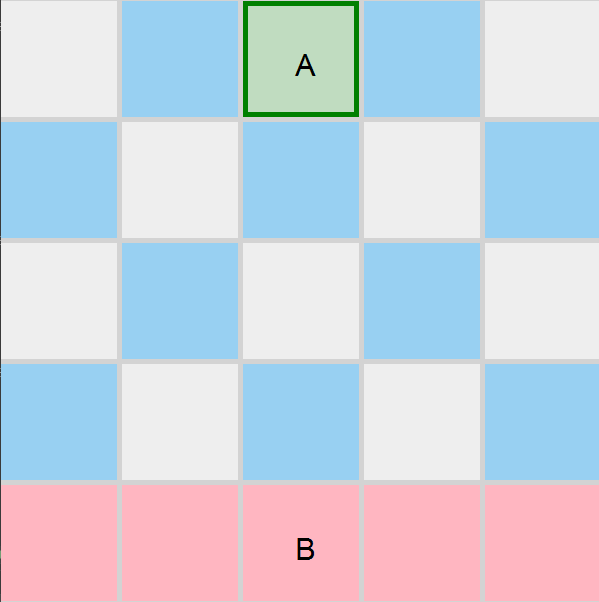
\includegraphics[scale=0.25]{../img/GameBoard/initial.png}
    \caption{A 5x5 game board}
    \label{fig:InitialGameBoard}
\end{figure}

As seen in figure \ref{fig:InitialGameBoard}, In the beginning, player A starts at cell (2, 0) and player B 
starts at cell (2, 4). A's goal is to reach the cells highlighted in pink. The gray areas between the cells
are grooves for wall placement.


\section{Notation}

There are no official notations for this game. However, some popular ones recognized by the Quoridor community
include \textbf{Glendenning's Notation} (\citep{Glendenning2002MasteringQ}) and the \textbf{Quoridor Strats Notation}
(\citep{website:COMMUNITY_NOTATION}). 
\par
Let $R = \{a, ..., i\}$ and $C = \{1, ..., 9\}$
\newline
Both notations follow the same principle of labelling each cell by $C_{ij}$ where $i \in R$ and $j \in C$.
\newline
Move $M$ and Wall $W$ are denoted algebraically, where
\par
$M(C_{ij}) = ij$ where $i \in R$ and $j \in C $,
\par
$W(C_{ij}) = ijD$ where $i \in R$, $j \in C$ and $D \in \{h, v\}$
\newline
\newline
The difference between the two notations is the way the walls are represented.

\begin{figure}[h]
    \begin{subfigure}{0.4\textwidth}
      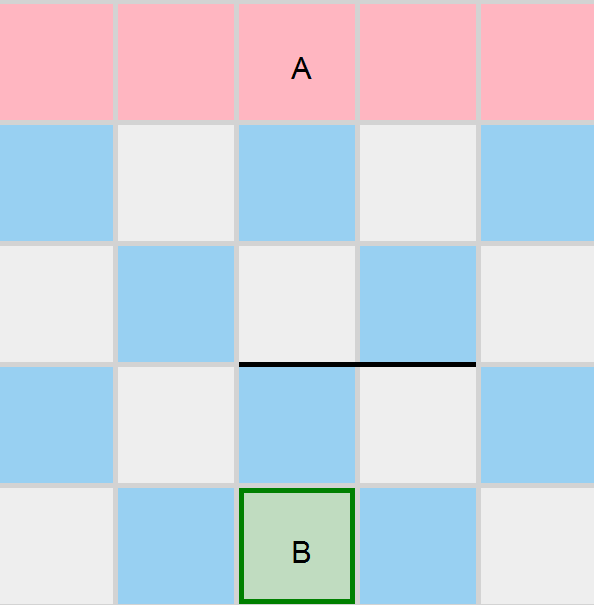
\includegraphics[width=\textwidth]{../img/GameBoard/wall_repr.png}
      \caption{Glendenning's Notation: \textbf{c3h}}
      \label{fig:NotationDifferentA}
    \end{subfigure}
    \hfill
    \begin{subfigure}{0.4\textwidth}
      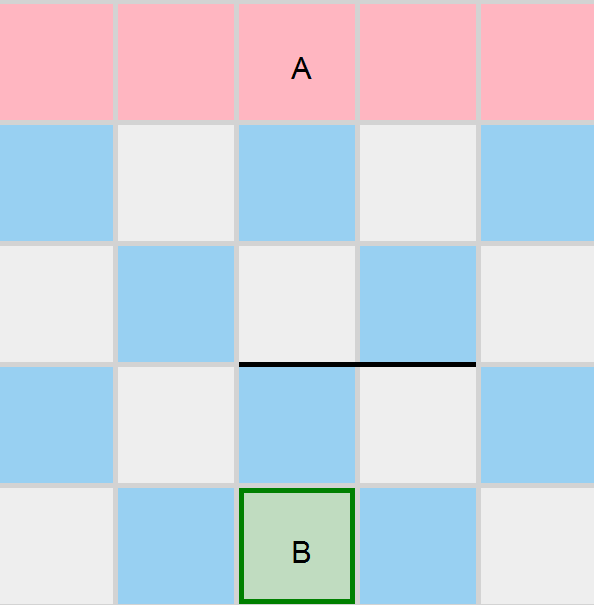
\includegraphics[width=\textwidth]{../img/GameBoard/wall_repr.png}
      \caption{Quoridor Strats Notation: \textbf{c4h}}
    \end{subfigure}
    \caption{Notation differences}
    \label{fig:WallNotationsDifferent}
\end{figure}

As seen in Figure \ref{fig:WallNotationsDifferent}, the difference lies in the point of reference of the wall.
In \textbf{Quoridor Strats Notation}, each wall coordinate is represented by the lower-left cell the wall
follows along, whereas in \textbf{Glendenning's Notation}, each wall is represented by the upper-left cell the
wall follows along.


Even though they are widely used, they are very easy to get confused with since they have the same wall representations,
and unless specified explicitly, it is difficult to tell which representation is being used.
\par
This is why I have decided to use a different representation for walls. Instead of vertical and horizontal wall
with respect to a cell, we define a direction explicitly.
\par
$W(C_{ij}) = ijD$ where $i \in R$, $j \in C$ and $D \in \{N, S, E, W\}$
\newline
Looking back at Figure \ref{fig:NotationDifferentA}, the walls can now be represented by \textbf{c4N}, i.e. a
Northern wall from the cell $C_{c4}$.

\pagebreak

\section {Rules}

\subsection{Wall placement rules}
\label{WallRules}

\begin{itemize}
    \item Walls cannot be placed diagonally.
    \item A placed wall must not completely block any player's path to victory. Each player must have at least
        one path to victory \textit{(See figure \ref{fig:WallBlockingMove})}
    \item A placed wall cannot intersect any of the previously placed walls.
    \item Walls cannot be placed along the edges of the board. Walls must be placed to create a barrier for
        exactly 4 cells
    \item  Every player possesses a limited supply of walls, and once they exhaust these walls, they are unable
        to place any additional ones. Consequently, the player is only allowed to maneuver their pawn on the
        board.
\end{itemize}

\begin{figure}[h]
    \begin{subfigure}{0.4\textwidth}
      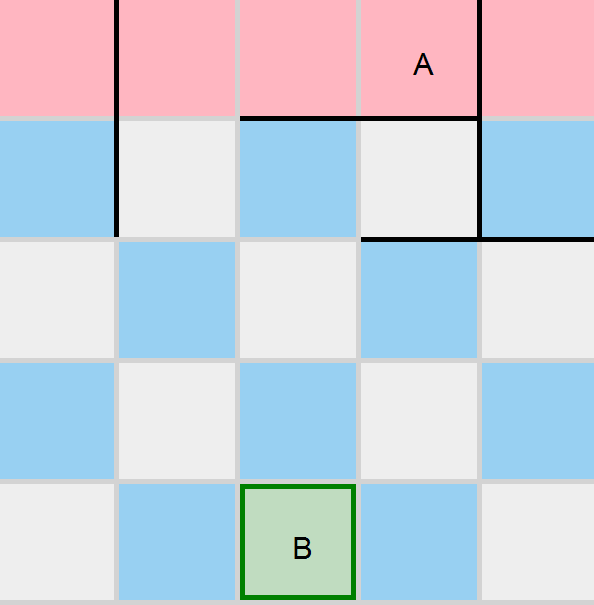
\includegraphics[width=\textwidth]{../img/GameBoard/arbitrary_state.png}
      \caption{Valid game state}
      \label{fig:ValidState}
    \end{subfigure}
    \hfill
    \begin{subfigure}{0.4\textwidth}
      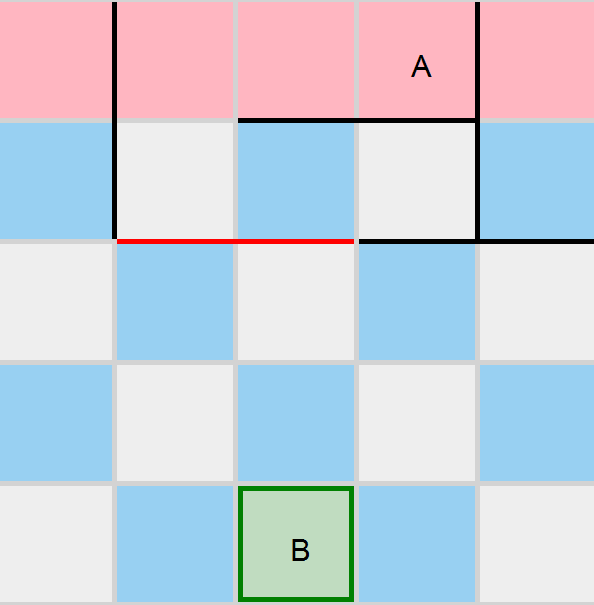
\includegraphics[width=\textwidth]{../img/GameBoard/invalid_wall.png}
      \caption{Invalid game state}
      \label{fig:WallBlocked}
    \end{subfigure}
    \caption{Example of an invalid wall placement}
    \label{fig:WallBlockingMove}
\end{figure}

The game state represented by Figure \ref{fig:ValidState} shows the situation after 5 turns, with it currently
being player B's turn to move. Since both \textbf{A} and \textbf{B} have viable paths to their respective goal
rows and all walls have been placed according to the rules (see \textit{Section \ref{WallRules}}),
the game state shown in Figure \ref{fig:ValidState} is considered valid.
\par
However, player B disrupts the rules by placing the red wall, violating the specified wall-placement rules
(see \textit{Section \ref{WallRules}}), consequently rendering the game state represented by
Figure \ref{fig:WallBlocked} invalid.

\pagebreak

\subsection{Player movement rules}
\label{PlayerMoveRules}
\begin{itemize}
    \item Players are allowed to move their pawn one unit at a time in the North, South, East, or West
        directions during their turn. Diagonal movements are not allowed.

    \item \textbf{Jump}
    \begin{itemize}
        \item If an opponent is at to the cell a player intends to move to, the player can jump over the
            opponent provided there is no wall between them or behind the opponent they intend to jump over.
            In the latter case, the player can jump to a cell on either side of the opponent's cell, given
            the cell is accessible from the opponent's cell.
        \item Players cannot jump over walls
        \item A Player is allowed to jump over multiple opponents as long as they adhere to the aforementioned
            conditions.
    \end{itemize}
\end{itemize}

\begin{figure}[h]
    \begin{subfigure}{0.2\textwidth}
      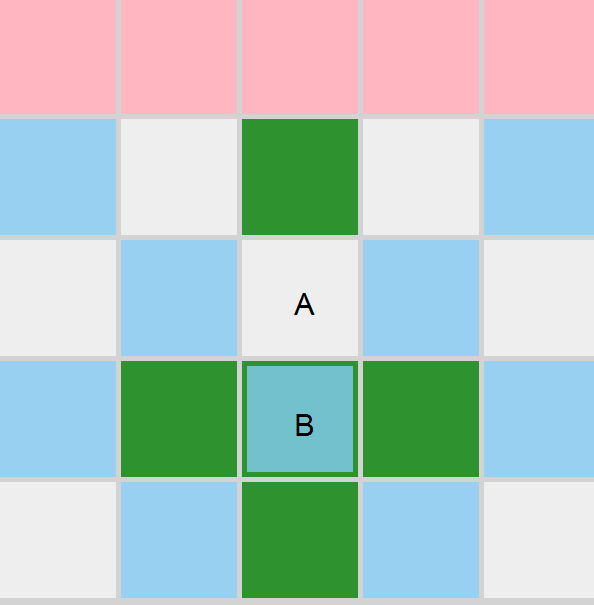
\includegraphics[width=\textwidth]{../img/GameBoard/move01.png}
    \end{subfigure}
    \hfill
    \begin{subfigure}{0.2\textwidth}
        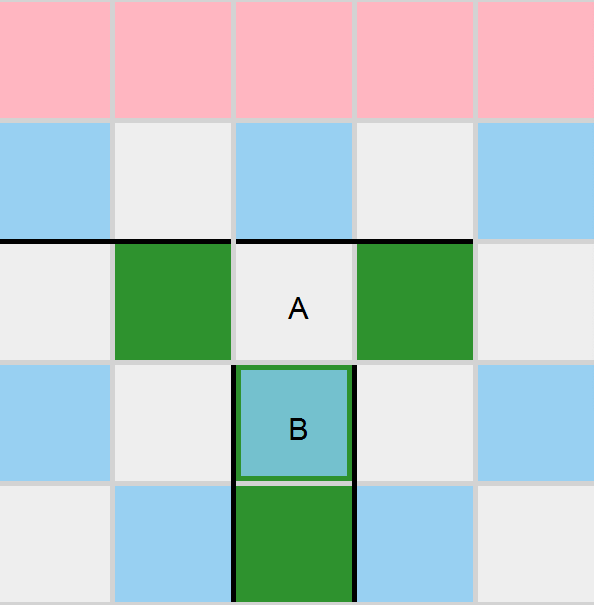
\includegraphics[width=\textwidth]{../img/GameBoard/move02.png}
    \end{subfigure}
    \hfill
    \begin{subfigure}{0.2\textwidth}
        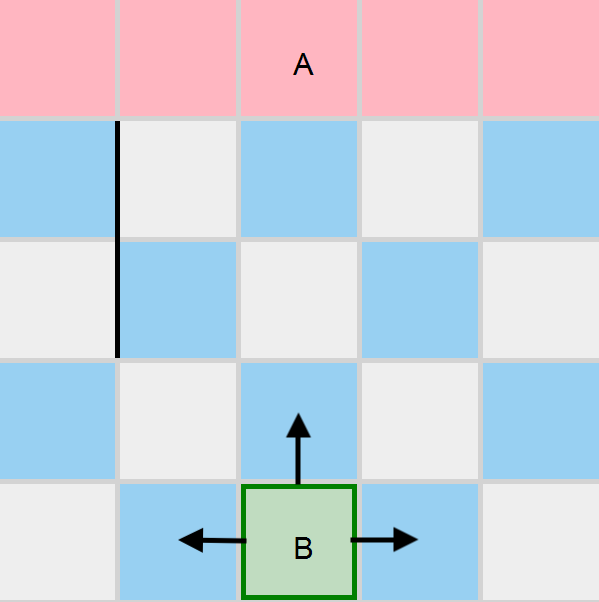
\includegraphics[width=\textwidth]{../img/GameBoard/move03.png}
    \end{subfigure}
    \hfill
    \begin{subfigure}{0.2\textwidth}
        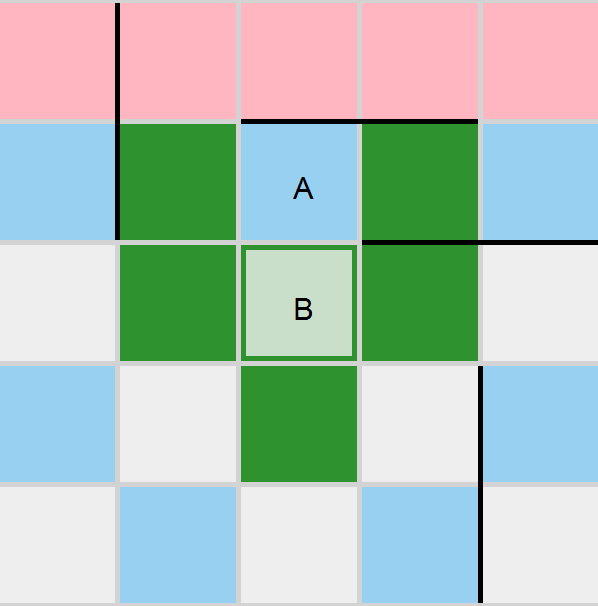
\includegraphics[width=\textwidth]{../img/GameBoard/move04.png}
    \end{subfigure}
    \caption{Examples of possible moves for player B in the game state}
    \label{fig:PossibleMoves}
\end{figure}
\chapter{Game Analysis}

\begin{figure}[h]
    \centering
    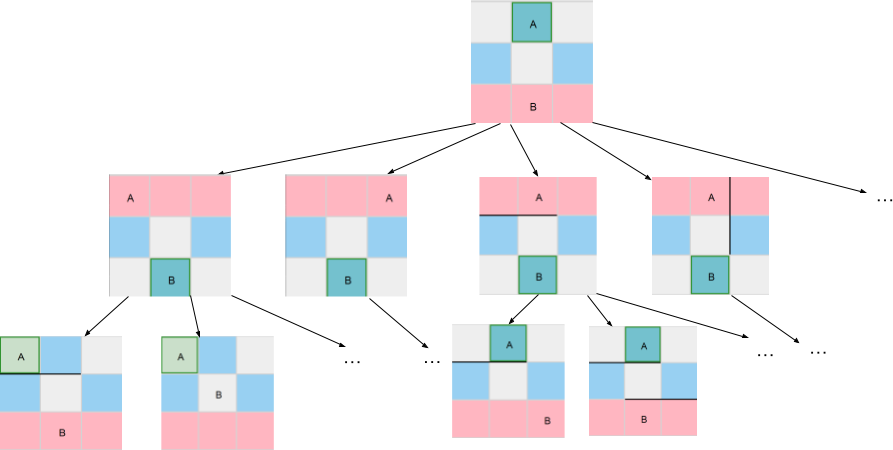
\includegraphics[scale=0.45]{../img/GameBoard/game_tree.png}
    \caption{A partial game tree for a 3x3 game board}
    \label{fig:GameTree}
\end{figure}
\chapter{Implementation}\label{Implementation}

In this chapter, we delve into the practical aspects of creating \gls{AI} agents capable of tackling abstract strategy games. The focus is on constructing adaptable interfaces that can be applied to a variety of games, ranging from the simplicity of Tic-tac-toe to the profound strategic depths of Go, with our primary case study being the game of Quoridor.

\gls{Csharp}, is selected as the language of choice, mainly for its robustness, versatility, and strong support for object-oriented programming paradigms. \gls{Csharp}'s rich feature set makes it an excellent tool for developing sophisticated \gls{AI} frameworks that require a blend of performance, maintainability and readability.

\section{Interfaces}
\label{game_interface_def}
The architecture of our implementation leverages interfaces, which specify a set of methods relevant to game mechanics. They form the backbone of our \gls{AI} systems, ensuring that the algorithms are versatile and can be adapted to new games with minimal changes to the underlying codebase. An example of such interface usage can be seen in Section \ref{TicTacToe}

Through the use of generic parameters \textbf{TPlayer}, \textbf{TMove}, and \textbf{TGame}, these interfaces offer a framework that is adaptable to various game entities such as players, moves, and game states.

Before describing the game-specific interfaces, we first introduce the generic \textbf{IAIStrategy\textless{}TMove, TGame, TPlayer\textgreater{}} interface, which acts as a common interface for all our \gls{AI} agents.
\begin{lstlisting}
interface IAIStrategy<TMove, TGame, TPlayer>
{
    string Name { get; }
    AIStrategyResult<TMove> BestMove(TGame game, TPlayer player);
}

class AIStrategyResult<TMove>
{
    double Value { get; set; }
    TMove BestMove { get; set; }
}
\end{lstlisting}
This interface provides a common property \textbf{Name}, a \texttt{string} representing the name of the agent, and a method \textbf{BestMove} that takes in a game and the current player in the game, and returns a tuple, \textbf{BestMove} (parametrized over generic type \textbf{TMove}) being the best move for the current player in the given game state and \textbf{Value}, a \texttt{double} type representing the value corresponding to the best move selected by the \gls{AI} agent.
For example, for the Minimax algorithm, the Value corresponding to the best move would be the state with the highest payoff function, which could be used for debugging purposes.
\\
The following interfaces are used within the \textbf{BestMove} method for each \gls{AI} agent, and are meant to be defined explicitly by the user within their game.

\begin{lstlisting}
interface IValidMoves<TMove>
{
    IEnumerable<TMove> GetValidMoves();
}
\end{lstlisting}

The \textbf{IValidMoves\textless{}TMove\textgreater{}} interface is the most fundamental interface used by (almost) all our \gls{AI} systems. Parametrized over the generic type \textbf{TMove}, this interface provides access to all valid moves (of a user-defined \textbf{TMove} type), e.g from the current game state, which our implemented \ac{AI} algorithms evaluate and find the best move.

\begin{lstlisting}
interface IPlayer<TPlayer>
{
    TPlayer CurrentPlayer { get; }
}

interface IOpponent<TPlayer>
{
    TPlayer Opponent { get; }
}
\end{lstlisting}

Since we are focussed on abstract \textbf{Two-player}, Zero-sum games, we also provide the \textbf{IPlayer\textless{}TPlayer\textgreater{}} and \textbf{IOpponent\textless{}TPlayer\textgreater{}} interfaces, both parametrized over the generic \textbf{TPlayer} type.
The \gls{MCTS} algorithm, for example, uses these interfaces during the simulation and back-propagation phases.
\begin{lstlisting}
TPlayer Simulation(TGame game)
{
    while(!game.HasFinished)
    {
        var move = _moveStrategy.BestMove(game, game.CurrentPlayer).BestMove;
        game.Move(move);
    }
    return game.Winner;
}
\end{lstlisting}
During the Simulation phase, the \gls{MCTS} algorithm uses e.g the Random agent, which implements the \textbf{IAIStrategy} interface, therefore providing access to the aforementioned \textbf{BestMove} method, which requires \textbf{CurrentPlayer} to be passed to it.

\begin{lstlisting}
void BackPropagation(Node<TMove, TPlayer, TGame> node, TPlayer winner)
{
    var current = node;
    while (current != null)
    {
        current.Count++;
        if (current.State.Opponent.Equals(winner))
            current.Wins++;

        current = current.Parent;
    }
}
\end{lstlisting}
Each node is expanded by making a move, and we keep a track of the player making the move in the node. After making the move in the game, we \textbf{Switch} the player turn. So the \textbf{CurrentPlayer} and \textbf{Opponent} gets switched too.

\begin{lstlisting}
interface IDeepCopy<T>
{
    T DeepCopy();
}
\end{lstlisting}
Although \gls{Csharp} has the \textbf{ICloneable\textless{}T\textgreater{}} interface provides a \textbf{T Clone()} method that we could use instead of our defined \textbf{IDeepCopy\textless{}T\textgreater{}} interface, the method we define leaves no room for ambiguity on shallow vs deep copying of relevant objects.
This method is used by e.g Parallel Minimax in order to ensure the original game state don't get changed by any means while exploring the game tree by making several moves.

\begin{lstlisting}
interface ITerminal
{
    bool HasFinished { get; }
}
\end{lstlisting}
Another important information for a game is whether the game reached the terminal state (win, loss, draw). This information helps update evaluations of game states and also notifies the algorithms to stop looking further. For example, in the Simulation phase of the \gls{MCTS} algorithm we described above, we see the usage of the \textbf{HasFinished} property. The Simulation phase performs moves until the game reaches a terminal state.

\begin{lstlisting}
interface IStaticEvaluation
{
    public double Evaluate(bool currentMaximizer);
}
\end{lstlisting}
The \textbf{IStaticEvaluation} interface computes the heuristic evaluation of the current game state, indicating the desirability of the state for the player who is currently maximizing or minimizing the game value. This is used by the \textbf{Minimax} algorithm to statically evaluate game states instead of exploring them when the specified depth has been reached.
\begin{lstlisting}
 MinimaxStep(TGame game, bool maximizingPlayer, int depth)
    if (depth <= 0 || game.HasFinished)
    {
        return game.Evaluate(maximizingPlayer);
    }
\end{lstlisting}
As we see from the base case of the recursive \textbf{MinimaxStep} method, we statically evaluate game states instead of recursing further and later compare them to find the best move.
\begin{lstlisting}
interface IMove<TMove>
{
    void Move(TMove move);

    void UndoMove(TMove move);
}
\end{lstlisting}
The \textbf{IMove\textless{}TMove\textgreater{}} interface is yet another fundamental interface that allows games to progress further. To further evaluate game states, \gls{AI} algorithms must make different moves from current game state, then run any evaluation function and make decisions based on that. The \textbf{Move} method provides access to do exactly that.\\
The \textbf{UndoMove} method complements the \textbf{Move} method in that the algorithms can track back to the original game state using the \textbf{UndoMove} method before returning the best move it found based on different game state evaluation.

\begin{lstlisting}
interface INeighbors<TMove>
{
    IEnumerable<TMove> Neighbors(TMove pos);
}
\end{lstlisting}
The \textbf{INeighbors\textless{}TMove\textgreater{}} interface yields the neighboring positions or states from a given position (parametrized using the generic \textbf{TMove} type) crucial for determining potential player actions. This is used by the \textbf{A*} algorithm to find the shortest path to the goal.

\begin{lstlisting}
interface IRandomizableMoves<TMove>
{
    public IEnumerable<TMove> RandomizableMoves();
}
\end{lstlisting}
The \textbf{IRandomizableMoves\textless{}TMove\textgreater{}} interface returns all the valid moves (that guide the current game state towards the terminal state) that can be made from the current state and can be used by the random agent.
In context of the Quoridor game, if we move randomly on each turn, there's a possibility of never reaching the goal row. So, we would instead like to have an option to place wall randomly, but move towards the goal. So, we define the \textbf{IRandomizableMoves} interface and return all possible walls that can be placed in the board, and use a different approach for pawn movements.


\section{Agents}

In this section, we discuss the generic \gls{AI} agent implementation, namely Random, Semi-Random, Minimax, A-Star, Monte Carlo Tree search, and describe how the aforementioned interfaces are used as building blocks for the algorithm.

\subsection{Random Agent}
We consider a random agent as a baseline for comparing the performance of the other implemented agents. 

The random agent uses the \textbf{IValidMoves\textless{}TMove\textgreater{}} interface to get a list of all valid moves, and then picks move at random. The class definition for the Random Strategy is given by:
\begin{lstlisting}
public class RandomStrategy<TMove, TGame, TPlayer>(int seed) :
    IAIStrategy<TMove, TGame, TPlayer>
        where TGame : IValidMoves<TMove>
\end{lstlisting}

As the Random Strategy implements the \textbf{IAIStrategy\textless{}TMove, TGame, TPlayer\textgreater{}} interface, it has a property \textbf{Name} of \texttt{string} type and the \textbf{BestMove(TGame game, TPlayer player)} method that returns the best move and the value that accompanies with it is the seed provided while initializing the random nubmer generator. The pseudocode for the Random agent is given below.

\begin{lstlisting}   
public string Name => "Random";

public AIStrategyResult<TMove> BestMove(
    TGame game, TPlayer player)
{
    //IValidMoves<TMove>
    var validMoves = game.GetValidMoves();

    var randIndex = random number between 0 and validMoves.Count();
    return { BestMove = validMoves[randIndex], Value = seed };
}
\end{lstlisting}

As described above, the Random Agent picks a move from the set of valid moves based on the \textbf{IValidMoves\textless{}TMove\textgreater{}} interface.

\subsection{Semi-Random agent}

There are cases where we want to return a random move, but we don't want the game to continue forever by the random agent possibly returning move that never end in a terminal state. In this case, we want to guide the random agent to produce a random move, but also make sure the game will terminate eventually.

The semi-random agent uses the \textbf{IRandomizableMoves\textless{}TMove\textgreater{}}. It also takes in a strategy to get the best move and then add it to the list of randomizable moves.

\begin{lstlisting}
public class SemiRandomStrategy<TGame, TMove, TPlayer> :
    IAIStrategy<TMove, TGame, TPlayer>
        where TGame : IRandomizableMoves<TMove>
\end{lstlisting}

Then, in the \textbf{BestMove} method, it firstly gets the list of moves that can be randomized, finds the best move from a list of non-randomizable move set and then produces a random move from these two. The pseudocode from the \textbf{Semi-Random} algorithm is given below:

\begin{lstlisting}
public TMove BestMove(TGame game, TPlayer player)
{
    //IRandomizableMoves<TMove>
    //these moves won't result in a possible infinite game
    possibleMoves = game.RandomizableMoves();

    //non-randomizable move. This move might create infinite game
    //loop if not used strategically, eg. pawn moves in Quoridor.
    nonRandomizableMove = _strategy.BestMove(game, player);

    //add the non-randomizable move to the list of all moves
    possibleMoves.Add(nonRandomizableMove);

    return random move from possibleMoves
}
\end{lstlisting}

Adding more context to the Quoridor example in the \textbf{IRandomizableMoves\textless{}TMove\textgreater{}} interface description in section \ref{game_interface_def}, the Semi-Random algorithm in Quoridor would process and return the best move the following way:

\begin{lstlisting}
//IRandomizable<TMove>
//No pawn placement positions here
unplaced_walls = game.GetRandomizableMoves();

//IPlayer.CurrentPlayer
//Shortest path to the goal row
best_pawn_move = AStar.BestMove(game, game.CurrentPlayer);

possible_moves = unplaced_walls + [best_pawn_move];
random_index = random nubmer from 0 to possible_moves;
return { BestMove = possible_moves[random_index], Value = random_seed };
\end{lstlisting}

This algorithm is especially useful for the Simulation step of the \gls{MCTS} algorithm as an approach to shorten the game length to reach the terminal state in context of Quoridor game.

\subsection{Minimax Agent}

Minimax agent is another agent that we have implemented in the game that provides the move to the agent based on minimax algorithm.

Mathematically, a minimax algorithm can be defined by the following equation:
\begin{equation}\label{eq:mmax}
    \bar{v}_i = \min_{a_{-i}} \max_{a_{i}} v_i (a_i, a_{-i})
\end{equation}
where,
\begin{subequations}
\begin{align}
    &i, -i = \text{index of the player of interest, opponent respectively} \\
    &a_i, a_{-i}= \text{action of the player of interest, opponent respectively} \\
    &v_i = \text{value function of player i} \\
    &\bar{v}_i = \text{minimax value of the player of interest}
\end{align}
\end{subequations}

As defined in the equation \eqref{eq:mmax}, the minimax algorithm comprises of two parts. The first part is maximizing part where the player chooses an action from a set of possible actions to maximize the evaluation of the game. Then, the player determines the subsequent action of the opponent to minimize the evaluation of the game. This is clarified further with the following example.

\begin{figure}
    \centering
    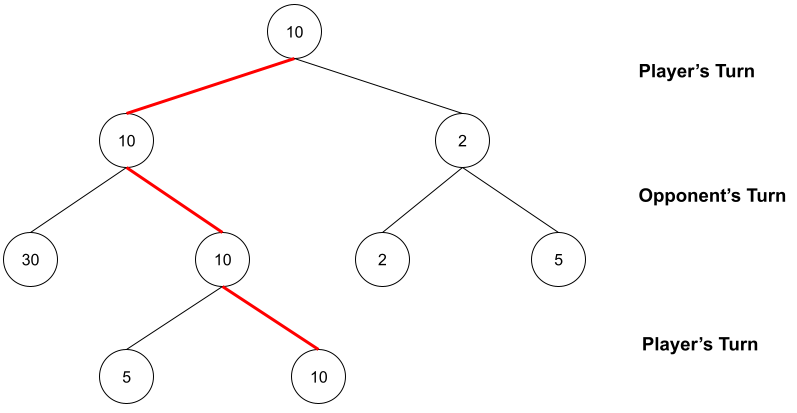
\includegraphics[width=\linewidth]{../img/Minimax1.png}
    \caption{Figure illustrating an exemplary game tree and decision based on minimax algorithm}
    \label{fig:minimax1}
\end{figure}

The Figure \ref{fig:minimax1} consists of nodes that define either player's or the opponent's actions. In our minimax implementation, we have considered an evaluation function as a linear combination of multiple features such as shortest distance to the goal and remaining number of walls. This is explained in detail in section \ref{sec:gameimplementation}. The numbers for each node Figure \ref{fig:minimax1} represent the evaluation of this function. For each action, there can be an evaluation where higher evaluation may mean it is favouring the player. For example, an action of the player causing two possible evaluations of 10 and 20 would mean the player would have higher advantage choosing the action leading to evaluation of 20. 

The minimax algorithm starts with a game tree with possible moves of the player and opponent. The evaluation of the leaf nodes positions are assigned, for example 5 and 10 in the figure. The player chooses a move to maximize the evaluation on their turn whereas the opponent wants to minimize the evaluation. The player chooses evaluation of 10 (between 10 and 5) on its turn and subsequently evaluation of 10 (between 10 and 30) in the opponent's turn. The red line shows the path the player determines as optimal leading to a decision choosing the the action labelled with evaluation of 10.


As the graph of a game can be large, one way to limit the search space for implementing the minimax algorithm is consider a depth-limited version of the algorithm. In this version, the algorithm only considers a part game tree with limited depth of the graph. Increasing the depth increases the accuracy of the decision at the cost of computational complexity. In terms of game, this depth may be equivalent to "looking ahead only a few moves".

In our implementation, the minimax algorithm is implemented with further optimizations including the alpha-beta pruning and the parallel version of the algorithm as described below:

\subsubsection{Alpha-beta pruning}

\begin{figure}[!ht]
    \centering
    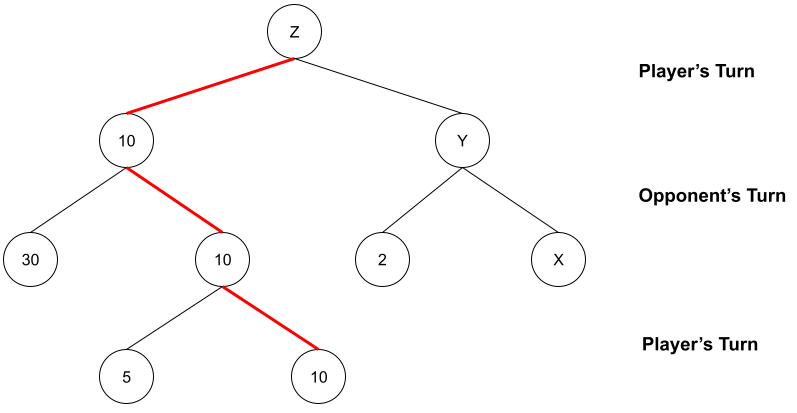
\includegraphics[width=\linewidth]{../img/Minimax2.png}
    \caption{Exemplary figure illustrating the alpha beta pruing for minimax algorithm}
    \label{fig:minimax2}
\end{figure}

In many cases, there may be the actions of the player in the search tree that can be evaluated worse than another action already evaluated. In such cases, where the better move or action has already been determined, it may not be useful to further evaluate the subsequent moves of the player and the opponent. Hence, the alpha-beta pruning reduces the game complexity by not further evaluating the branches of the node with evaluation worse than what has already been determined with another node.

As its name suggests, the alpha beta algorithm maintains two values, alpha and beta values. The alpha value stores the minimum score the player is assured to get while the beta value records the maximum score the opponent is assured to get. Whenever the evaluation of the minimum score of the player is higher than the maximum score after the subsequent move of the opponent (or in other words alpha $>$ beta), the alpha-beta pruning algorithm stops evaluating the opponents position. This reduces the number of nodes in the search tree and hence reduces the complexity of the minimax algorithm.

In Figure \ref{fig:minimax2}, if the player determines that 
\begin{equation}
    Z = max (10, Y) = max (10,  min (2, X)),
\end{equation}
the value of X does not influence the value of $Y$ or $Z$ as $Y = min(2, X) \leq 2$ and hence $Z = max(10, \leq 2) = 10$. In this case, the player may not evaluate the branch $X$ or branch $Y$ further reducing the game tree and hence the computational complexity of the algorithm. 


The minimax algorithm (and the alpha-beta pruning optimization of it)  uses the \textbf{IValidMoves\textless{}TMove\textgreater{}} interface to get a list of all moves, \textbf{IMove\textless{}TMove\textgreater{}} interface to perform moves, get a static evaluation (therefore needing the \textbf{IStaticEvaluation} interface) of the game state and undo moves. It also requires the \textbf{ITerminal} interface to check if the game reached the terminal state, and an access to the \textbf{IPlayer\textless{}TPlayer\textgreater{}} interface, especially during the static evaluation in order to know which player to evaluate the board for.

The class definition for Minimax would then be the following:

\begin{lstlisting}
 public class Minimax<TPlayer, TMove, TGame>(int Depth) :
    IAIStrategy<TMove, TGame, TPlayer>
        where TGame :  ITerminal, IMove<TMove>, IStaticEvaluation,
            IValidMoves<TMove>, IPlayer<TPlayer>
\end{lstlisting}

Below, we list the implementation of the minimax algorithm with alpha beta pruning implementation:

\begin{lstlisting}
public TMove MinimaxStep(
    TGame game, int depth, bool maximizingPlayer, int alpha, int beta) {
    
    // return static evaluation if depth reached or game over
    // IStaticEvaluation

    bestMove = maximizingPlayer ? MinValue : MaxValue;
    
    // IValidMoves<TMove>
    foreach(var move in game.GetValidMoves())
    {
        // IMove<TMove>
        game.Move(move);
        result = MinimaxStep(game, depth - 1, !maximizingPlayer);
        // IMove<TMove>
        game.UndoMove(move);

        if (maximizingPlayer)
        {
            if (result.Value > bestMove.Value)
            {
                bestMove.BestMove = move;
                bestMove.Value = result.Value;
            }
            if (bestMove.Value > beta)
                break;

            alpha = Math.Max(alpha, bestMove.Value);
        }
        else
        {
            if (result.Value < bestMove.Value)
            {
                bestMove.BestMove = move;
                bestMove.Value = result.Value;
            }
            if (bestMove.Value < alpha)
                break;

            beta = Math.Min(beta, bestMove.Value);
        }
    }
    return bestMove;
}
\end{lstlisting}

We have implemented a recursive minimax agent with alpha-beta pruning that is depth limited. The algorithm alternates with the variable \textit{maximizingPlayer} being 1 and 0 in each step indicating whether its the player's turn or the opponent's. In each case, the player determines the evaluation of the branch in the variable \textit{result} and sets the node as the best if it is the maximum (if player's turn) or minimum (if opponent's turn).

In the above implementation, the parameter depth is introduced to only consider the depth limited version of the algorithm, and alpha and beta variable limit the search space of the nodes in game tree.

\subsubsection{Parallel minimax}
Another way to improve the time complexity of the minimax algorithm is to parallelize the algorithm. The minimax algorithm involves in evaluating multiple nodes of the game tree. The way to parallelize such algorithm is to run different processes, in this case, evaluation of the position associated with different nodes, in different threads. This ensures that even though computational complexity may remain the same, the time complexity of the algorithm is distributed over multiple threads and possibly multiple processors.

The above defined methods to reduce the computational complexity of the minimax algorithm can be combined together. For example, the minimax algorithm can be depth limited and/or run with alpha-beta pruning and/or run in parallel as shown in the following pseudocode:

\begin{lstlisting}
Parallel.ForEach(validMoves, (move, loopState) =>
{
    //IDeepCopy<T>
    var clonedGame = game.DeepCopy();
    clonedGame.Move(move);

    var result = ParallelMinimaxStep(clonedGame, alpha, beta, depth - 1, !maximizingPlayer);

    lock (_lock)
    {
        bestMove = Update(result, bestMove);
    }
});
return bestMove;
\end{lstlisting}


\textbf{Parallel Minimax} additionally requires the \textbf{IDeepCopy\textless{}T\textgreater{}} interface to ensure the original game state doesn't get altered in any way. The other two variants of Minimax algorithms were only using the  \textbf{IMove\textless{}TMove\textgreater{}} interface since one thread was responsible for changing the game state sequentially so undoing a move would cancel out the applied move effectively.

\subsection{Monte-Carlo tree search agent}

\begin{figure}[!ht]
    \centering
    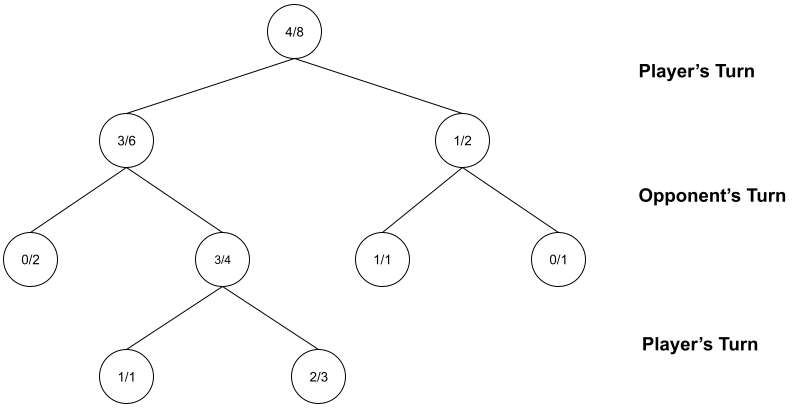
\includegraphics[width = \linewidth]{../img/MCTS1.png}
    \caption{Figure illustrating an iteration of the MCTS algorithm}
    \label{fig:MCTS1}
\end{figure}

\ac{MCTS} is a heuristic algorithm for searching the game tree based on Monte-Carlo simulations. As shown in Figure \ref{fig:MCTS1}, \gls{MCTS} algorithm determines the best path to the destination node in the game tree based on multiple trial runs through the game tree. In the figure, each node is labelled with a fraction where the denominator represents the total number of game runs through the node and the numerator represents the total number of wins for the player. For example, the game is simulated a total of 8 times in the example where the player wins 4 of the runs. The player wins 3/6 when taking an action while 1/2 when taking another action and so on.

The \gls{MCTS} algorithm builds upon the following framework:
\begin{enumerate}
    \item \textbf{Selection:} This step involves the algorithm choosing a move based on either a good move determined in previous iterations or a exploratory new move. For example, in figure \ref{fig:MCTS1}, in the first player's turn, an action gives 3/6 chances of winning based on previous iterations whereas another gives 1/2 winning chances. The player selects a node that has highest possibility of winning, which in this case is equal. The player can also choose a new move that may be already explored to avoid not exploring further options.
    \item \textbf{Expansion:} This step involves the algorithm to add a new node to the game tree determined during the selection process. A node can simply be a valid move starting from the node from where no simulation step has been played out. In figure \ref{fig:MCTS2}, an unevaluated option (e.g., node inside the dotted box) is explored and simulated.
    \item \textbf{Simulation:} This step involves the agent playing out the game using policy. One of the policies can simply be a random policy (e.g., choosing a move based on certain distribution).
    \item \textbf{Back propagation:} Finally, based on the simulation step, this step involves in the algorithm updating the nodes. In figure \ref{fig:MCTS2}, the red arrows show the back propagation step as a result of exploration and simulation step where the probabilities or the weights of the nodes are updated as a result of exploration and simulation steps.
\end{enumerate}

\begin{figure}[!ht]
    \centering
    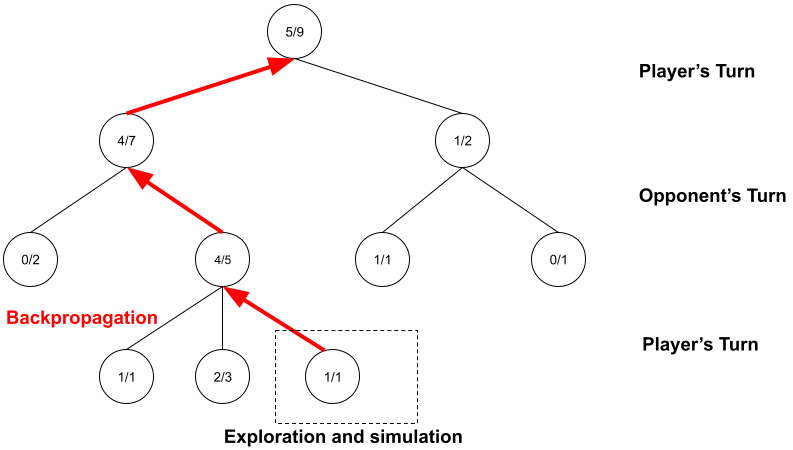
\includegraphics[width=\linewidth]{../img/MCTS2.png}
    \caption{Figure illustrating steps 2, 3, and 4 of the MCTS algorithm}
    \label{fig:MCTS2}
\end{figure}

The advantage of \gls{MCTS} algorithm over the minimax algorithm is that the \gls{MCTS} algorithm does not require any evaluation function as the weights are determined based on multiple simulation runs. On the contrary, the \gls{MCTS} algorithm requires multiple runs through the game to determine the weights.

\begin{lstlisting}
    public class MonteCarloTreeSearch<TMove, TGame, TPlayer> : IAIStrategy<TMove, TGame, TPlayer>
        where TGame : IMCTSGame<TGame, TMove, TPlayer>
        where TPlayer : IEquatable<TPlayer>
    {
    (*@{\hspace*{.5cm}\vdots}@*)    

        public AIStrategyResult<TMove> BestMove(TGame game, TPlayer player)
        {
            (*@{\hspace*{.5cm}\vdots}@*)
            for (int i = 0; i < _simulations; i++)
            {
                var selectedNode = Selection_Expansion(root);
                var winner = Simulation(selectedNode.State.DeepCopy());
                BackPropagation(selectedNode, winner);
            }
            (*@{\hspace*{.5cm}\vdots}@*)
        }

        private Node<TMove, TPlayer, TGame> Selection_Expansion(Node<TMove, TPlayer, TGame> node)
        {
            (*@{\hspace*{.5cm}\vdots}@*)
        }

        private TPlayer Simulation(TGame game)
        {
            (*@{\hspace*{.5cm}\vdots}@*)
        }

        private void BackPropagation(Node<TMove, TPlayer, TGame> node, TPlayer winner)
        {
            (*@{\hspace*{.5cm}\vdots}@*)        
        }
\end{lstlisting}

As described in the above code snippet, for \gls{MCTS} algorithm, the simulation is run \textit{${\_}simulations$} times and in each step, the game runs the four described steps. The best strategy is defined based on the Monte-Carlo runs and the determined final weights in the graph.

\subsection{A-Star agent}
A-Star is a search algorithm for traversing from the source node to the destination node while minimizing the cost function. The cost function, or "f" score, for a node depends on two components "g" value and "h" value. "g" value represents the distance from the source node to the node and "h" value represents the cost of the path from the node to the destination node, often defined by a heuristic. Mathematically,
\begin{equation}
    f = g + h
\end{equation}

We begin by describing the \textbf{IPlayer\textless{}TPlayer\textgreater{}} interface as follows:
\begin{lstlisting}
public interface IAStarPlayer<TMove>
{
    TMove GetCurrentMove();
    bool IsGoal(TMove move);
    double CalculateHeuristic(TMove move);
}
\end{lstlisting}
It is parametrized over the generic \textbf{TMove} type. The first method \textbf{TMove GetCurrentMove()} provides the current user-defined position (of type TMove). This could be e.g position in the game board.\\
The \textbf{IsGoal(TMove move)} method checks if the new move is a goal, i.e the player's goal move. E.g in context of Quoridor, where \textbf{Vector2} is used as \textbf{TMove}, each player has a \textbf{IsGoal(Vector2 pos)} that checks if the position is one of player's goal row.\\
The \textbf{CalculateHeuristic(TMove move)} is the heuristic function - the cost of the cheapest path from the current position to the goal. In Quoridor, for example, we use \textbf{Manhattan Distance} as the heuristic.\\
Suppose player $P$ is at at cell $C_{xy}$ and player $Q$ starts at cell $C_{ab}$, and let $n$ be the Quoridor board dimension.\\
Player $P$'s goal is to reach row $n$ regardless of the column it is at, and Player $Q$'s goal is to reach row $1$.
So, the heuristic function for player $P$, $H_P$ is given by
\begin{equation}
\label{eq:playerPHeuristic}
    H_P = | n - x |
\end{equation}
and the heuristic function for player $Q$, $H_Q$ is given by
\begin{equation}
\label{eq:playerQHeuristic}
    H_Q = a
\end{equation}

Before we describe the class signature for the \textbf{A*} algorithm, we would want the user-defined \textbf{TMaze} type to implement the \textbf{INeighbors\textless{}TMove\textgreater{}} interface to get access to neighboring moves (e.g positions), given a move (or position).

\begin{lstlisting}
public class AStar<TMove, TMaze, TPlayer>
    where TPlayer : IAStarPlayer<TMove>
    where TMaze : INeighbors<TMove>
\end{lstlisting}

\begin{lstlisting}
public AIStrategyResult<TMove> BestMove(TMaze maze, TPlayer player)
{
    openSet = { start }
    var closedSet =  { }

    while (openSet is not empty)
    {
        nodeWithLowestFscore = node in openset with lowest f-score value

        //IAStarPlayer<TMove>
        if player.IsGoal(nodeWithLowestFScore):
            return nodeWithLowestFScore

        closedSet.Add(nodeWithLowestFscore);
        openSet.Remove(nodeWithLowestFscore);
        
        //INeighbors<TMove>
        foreach (neighbor in maze.Neighbors(nodeWithLowestFScore))
        if (!openSet.Contains(neighbor) || neighborNode.G < G)
            {
                neighbor.G = G;
                //IAStarPlayer<TMove>
                neighbor.H = player.CalculateHeuristic(neighbor);
                neighbor.F = G + neighbor.H;
            }
    }
\end{lstlisting}

The A-star algorithm starts by maintaining two sets \textit{openSet} and \textit{closedSet}. \textit{openSet} consists of nodes with children not yet visited and \textit{closedSet} consists of nodes with children nodes explored already. The node with lowest cost function ("f" score) is explored and marked as the \textit{currentNode} from the \textit{openSet}. Subsequently, the 'f' scores of the neighbours of the \textit{currentNode} is calculated. This algorithm runs until the destination node in the tree is reached.

\section{Generalization of AI interface to other games}
\label{TicTacToe}

In this section, we demonstrate how seamless it is to integrate the \gls{AI} agents with our implementation to other games. We will use an example to integrate our interface to the tic-tac-toe game for this purpose.

The interfaces with our implementation as described earlier  are parametrized over 3 generic types, namely TGame, TMove and TPlayer. For Tic-tac-toe, we will use the \textit{int} type for TMove and TPlayer parameteters. For TGame, we will use the \textbf{TicTacToe} class type.

\begin{lstlisting}
public class TicTacToe :
    ITerminal, //used by Minimax, used by MCTS
    IValidMoves<int>, //Minimax, MCTS
    IMove<int>, //Minimax, MCTS
    IPlayer<int>, //Minimax, MCTS
    IOpponent<int>, //MCTS
    IDeepCopy<TicTacToe>, //MCTS
    IWinner<int>, //MCTS
    IStaticEvaluation //Minimax
\end{lstlisting}

For the Tic-Tac-Toe game, we will need a 3x3 array representing the game board, and a property turn that represents which player's turn it currently is. Turn therefore will have 2 values, 1 and 2 representing player 1 and player 2 respectively.

\begin{lstlisting}
private int[,] Cells = new int[3, 3];
private int turn = 1; // 1 -> p1, 2 -> p2
\end{lstlisting}

The game board, represented by \texttt{Cells} property, is initially all zeros. Over the course of the game, it will contain values 0, 1 or 2.

We will now implement all the interfaces above. We start by implementing the \textbf{IValidMoves\textless{}int\textgreater{}} iterface. To get all the valid locations, i.e Cells marked by 0, we can encode the Cell's i and j position by the following equation
\begin{equation}
\label{eq:Move}
    Move(C_{ij}) = i + 3 * j
\end{equation}

As an example, consider the cell $C_{1,2}$. From equation \ref{eq:Move}, we have that $Move(C_{1,2}) = 1 + 3 * 2 = 7$.

\begin{lstlisting}
public IEnumerable<int> GetValidMoves() {
    for(int i =  0; i < 3; i++)
        for (int j = 0; j < 3; j++)
            if (Cells[i, j] == 0)
                yield return i + 3 * j;
}
\end{lstlisting}

We now write a method \textit{Place} that takes in two arguments, move and mark, move being an integral value repesented by equation \ref{eq:Move}, and mark being one of 0, 1, 2. 1 and 2.
On each placement, we can also retrieve the winner(if any) and get information on whether the game terminated, so we implement both the \textbf{ITerminal.HasFinished} and \textbf{IWinner.Winner} properties. To check if the game has finished we check if 3 adjacent sides of the game board are filled by the same player. These include diagonals too.
We define \textbf{Winner} to hold 4 possible values - 1 and 2 indicating player 1 and player 2 victory respectively, 0 indicating a draw and -1 indicating that the game is still in progress.
Before all these, we firstly need to decompose the move we encoded by equation \ref{eq:Move} to i and j values. To do so from given move $Move(C_{ij})$, we can use the following equations:
\begin{equation}
    i = Move(C_{ij}) \mod 3
\end{equation}
\begin{equation}
    j = \frac{Move(C_{ij})}{3}
\end{equation}
We then place one of 'X' or 'O' signs, (or remove them if we want to undo the last action), check if any player won, and if not, switch turns.

\begin{lstlisting}
public bool HasFinished => CheckWin();

// 0 draw, 1 -> p1, 2 -> p2, -1 game in progress
private int _winner = -1; 

public int Winner => _winner;

private void Place(int move, int item) {
    int i = move % 3;
    int j = move / 3;
    Cells[i, j] = item;
    CheckWin();
    turn = turn % 2 + 1;
}

void CheckWin() {
    //check all 3 consecutive adjecent squares (including
    //diagonals), and return true if they're filled by the
    //same player.
    // update the _winner variable based on this
}

\end{lstlisting}

We can then implement the \texttt{Move} and \texttt{UndoMove} methods. Both these methods use the \texttt{Place} method.
We also switch turns after a successful Move/UndoMove operation.
\begin{lstlisting}
 public void Move(int move) {
    Place(move, turn);
}

public void UndoMove(int move) {
    Place(move, 0);
}
\end{lstlisting}

We also need to implement the \texttt{CurrentPlayer} and \texttt{Opponent} properties implemented by the \textbf{IPlayer} and \textbf{IOpponent} interfaces respectively. We simply use the value held by the \textbf{turn} variable in our implementation to return it. The \textbf{turn} variable holds the index of the current player, so for the opponent, we simply return the value not held by the \textbf{turn} variable.

\begin{lstlisting}
public int CurrentPlayer => turn;

public int Opponent => turn % 2 + 1;    
\end{lstlisting}

To have the Tic-Tac-Toe implementation work smoothly with the Minimax algorithm, we also implement the \textbf{IStaticEvaluation.Evaluate()} method.
\begin{lstlisting}
public double Evaluate ( bool currentMaximizer ) {
    if ( _winner == CurrentPlayer ) return 1.0;
    if ( _winner == Opponent ) return -1.0;
    return 0.0;
}
\end{lstlisting}

Finally, we implement the \textbf{IDeepCopy} interface. This interface is used by the \gls{MCTS} algorithm, especially during the simulation phase so as to not change the original game state or properties references in any way possible.

\begin{lstlisting}
public TicTacToe DeepCopy() {
    var t = new TicTacToe();
    //shallow copy of struct(int in our case) is
    //fine since no reference is copied
    t.Cells = (int[,])Cells.Clone();
    t.turn = turn;
    return t;
}
\end{lstlisting}

We can now use the Minimax, Monte Carlo Tree Search, Minimax Alpha-beta pruning, Parallel Minimax Alpha-beta pruning, Random agents to play the game of tic-tac-toe. For example:

\begin{lstlisting}
var tt = new TicTacToe();

//MinimaxABPruning<TPlayer, TMove, TGame>
var minimaxABagent = new MinimaxABPruning<int, int, TicTacToe>(...);

//MonteCarloTreeSearch<TMove, TGame, TPlayer>
var mctsAgent = new MonteCarloTreeSearch<int, TicTacToe, int>(...);

minimaxBestMove = minimaxABAgent.BestMove(tt, tt.turn).BestMove;
tt.Move(minimaxBestMove);

mctsBestMove(tt, tt.turn).BestMove;
tt.Move(mctsBestMove);
\end{lstlisting}

This way, we can play the Tic-Tac-Toe game between 2 smart or trivial agents until the game finishes.

\section{Quoridor Game Implementation}\label{sec:gameimplementation}

\begin{figure}[!ht]
    \centering
    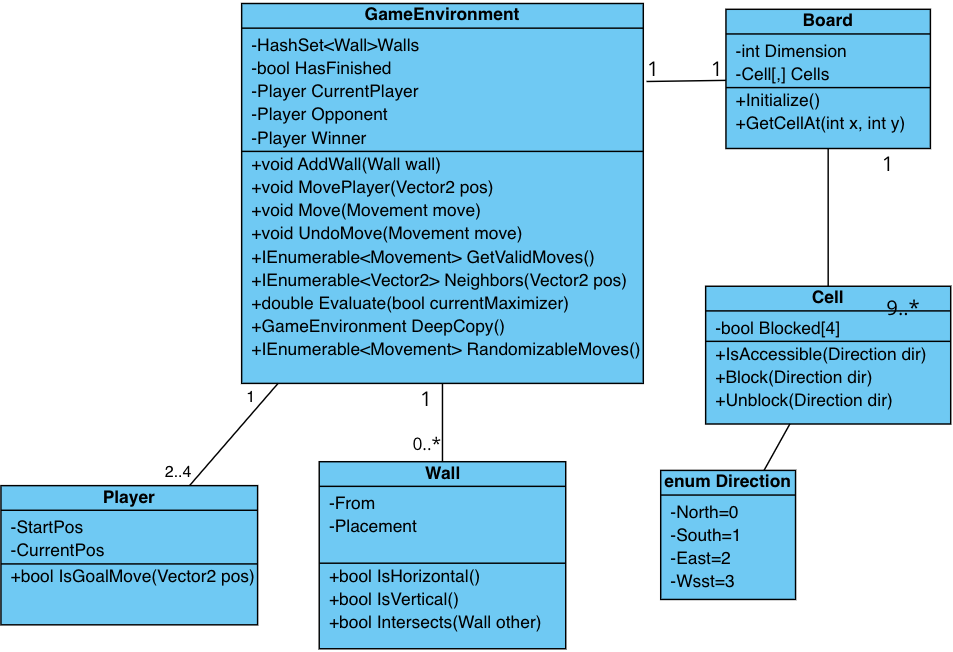
\includegraphics[width=.95\linewidth]{../img/uml_core.png}
    \caption{A UML diagram depicting relationship in the core library}
    \label{fig:core_uml}
\end{figure}

As seen in figure \ref{fig:core_uml}, the \texttt{GameEnvironment} class implements all interfaces necessary for \gls{AI} integration.

In contrast to the \textbf{Tic-Tac-Toe} implementation we saw earlier in section \ref{TicTacToe} where \texttt{int} type was used for the \texttt{TMove} parameter, we use a reference type \texttt{Movement} for the \texttt{TMove} parameter, since we need to consider wall placement and player movement, which is difficult to encode and decode as integral values.

\begin{lstlisting}
public abstract class Movement{}

public class Vector2 : Movement{...}

public class Wall : Movement{...};
\end{lstlisting}

This approach makes it easier to identify movement types and therefore easily perform Move/Unmove operations on the game and much more.

We will now describe the core elements of the interfaces that we integrated for this game.

\begin{lstlisting}
public IEnumerable<Movement> GetValidMoves() {
    List<Vector2> neighborMoves;
    //Populate the moves based on whether the neighboring
    //cells are accessible from the cell the current player
    //is in

    List<Wall> possibleWalls;
    //Populate the available wall list. We don't include
    //already placed walls/walls intersecting with already
    //placed walls

    return neighborMoves.Concat(possibleWalls);
}
\end{lstlisting}

Also, as described earlier, for the move and unmove operations, we do not need to decipher the movement by a pre-defined rule like we did in section \ref{TicTacToe}. We can easily check the underlying type of the abstract Movement type and do operations accordingly.

\begin{lstlisting}
public void Move(Movement move) {
    if (move is Vector2 v2) {
        MovePlayer(v2);
    }
    if (move is Wall wall) {
        AddWall(wall);
    }
    //change turn
}
\end{lstlisting}

Assume a Quoridor game instance of 2 players $P$ and $Q$, with $P$ starting at cell $C_{1c}$ and $Q$ starting at cell $C_{Nc}$, where $N$ is the dimension of the game board.\\
Suppose $P$ is at cell $C_{xy}$ and $Q$ is at cell $C_{uv}$ at an arbitrary game state $G_s$, and let $S_P$ be the shortest path from $C_{xy}$ to $C_{N*}$ and let $S_Q$ be the shortest path from $C_{uv}$ to $C_{0*}$.\\
Let $W_P$ denote the number of walls left for player $P$ and let $W_Q$ denote the number of walls left for player $Q$ at state $G_s$.

Then, the static evaluation function for player for player $P$, $F_P$ in game state $G_s$ is given by:

\begin{equation}
    F_P = S_P - S_Q + W_P - W_Q
\end{equation}

So, for the static evaluation function, we consider the following 4 features:
\begin{itemize}
    \item Shortest distance to goal for player P
    \item Shortest distance to goal for player Q
    \item Number of walls left for player P
    \item Number of walls left for player Q
\end{itemize}

\subsection{Project Structure}

The solution consists of six fundamental projects, each written in \gls{Csharp}.

\begin{itemize}
    \item \textbf{Quoridor.Core}\\
        This library project contains the core game logic for Quoridor, and implements all interfaces to allow \gls{AI} algorithms to run.
        
    \item \textbf{Quoridor.AI}\\
        This library project includes all the fundamental interfaces and a generic \gls{AI} algorithms implemented using these interfaces.

    \item \textbf{Quoridor.Common}\\
        This library project includes all common helpers, such as XML parser helper, logging helper, etc.

    \item \textbf{Quoridor.Tests}\\
        This NUnit test project includes all unit tests for robust development.

    \item \textbf{Quoridor.ConsoleApp}\\
        A CLI tool that runs simulations and allows user to play against an opponent with a visual interface.

    \item \textbf{Quoridor.DesktopApp}\\
        A WinForms application that allows user to play against one another or against various \gls{AI}.
\end{itemize}

These projects are inter-connected by references. For example from figure \ref{fig:proj_dep}, \textbf{Quoridor.AI} is a standalone library that contains all the interfaces, which is referenced by all other projects.
All project dependency structures are depicted in figure \ref{fig:proj_dep}.

\begin{figure}[!ht]
    \centering
    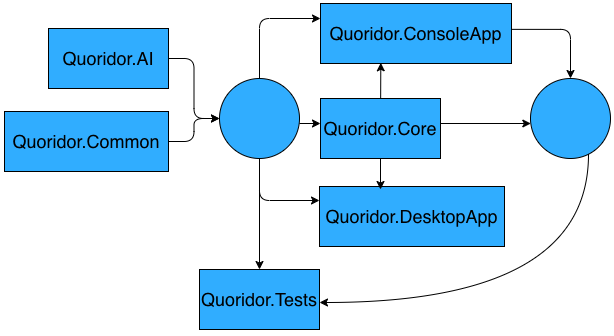
\includegraphics[width=.95\linewidth]{../img/project_structure.png}
    \caption{Quoridor project dependency diagram}
    \label{fig:proj_dep}
\end{figure}

\chapter*{Conclusion}
\addcontentsline{toc}{chapter}{Conclusion}


%%% Bibliography
%%% Bibliography (literature used as a source)
%%%
%%% We employ bibTeX to construct the bibliography. It processes
%%% citations in the text (e.g., the \cite{...} macro) and looks up
%%% relevant entries in the bibliography.bib file.
%%%
%%% The \bibliographystyle command selects, which style will be used
%%% for references from the text. The argument in curly brackets is
%%% the name of the corresponding style file (*.bst). Both styles
%%% mentioned in this template are included in LaTeX distributions.

\bibliographystyle{plainnat}    %% Author (year)
% \bibliographystyle{unsrt}     %% [number]

\renewcommand{\bibname}{Bibliography}

%%% Generate the bibliography. Beware that if you cited no works,
%%% the empty list will be omitted completely.

\bibliography{bibliography}

%%% If case you prefer to write the bibliography manually (without bibTeX),
%%% you can use the following. Please follow the ISO 690 standard and
%%% citation conventions of your field of research.

% \begin{thebibliography}{99}
%
% \bibitem{lamport94}
%   {\sc Lamport,} Leslie.
%   \emph{\LaTeX: A Document Preparation System}.
%   2nd edition.
%   Massachusetts: Addison Wesley, 1994.
%   ISBN 0-201-52983-1.
%
% \end{thebibliography}


%%% Figures used in the thesis (consider if this is needed)
\listoffigures

%%% Tables used in the thesis (consider if this is needed)
%%% In mathematical theses, it could be better to move the list of tables to the beginning of the thesis.
\listoftables

%%% Abbreviations used in the thesis, if any, including their explanation
%%% In mathematical theses, it could be better to move the list of abbreviations to the beginning of the thesis.
\chapwithtoc{List of Abbreviations}
\printglossaries


%%% Attachments to the bachelor thesis, if any. Each attachment must be
%%% referred to at least once from the text of the thesis. Attachments
%%% are numbered.
%%%
%%% The printed version should preferably contain attachments, which can be
%%% read (additional tables and charts, supplementary text, examples of
%%% program output, etc.). The electronic version is more suited for attachments
%%% which will likely be used in an electronic form rather than read (program
%%% source code, data files, interactive charts, etc.). Electronic attachments
%%% should be uploaded to SIS and optionally also included in the thesis on a~CD/DVD.
%%% Allowed file formats are specified in provision of the rector no. 72/2017.
\appendix
\chapter{Attachments}

\section{First Attachment}

\openright
\end{document}
